\section{Curves}

\subsection{Kurve in der Ebene}

\textbf{Explizite Darstellung} \\
$\gamma : [a,b] \rightarrow \mathbb{R} , x \mapsto y = f(x)$ \\
\textit{Kreis: \\oberer Halbkreis $\sqrt{r^2 - x^2}$ \\ unterer Halbkreis $\sqrt{r^2 - x^2}$} \\
\\
\textit{(Implizite Darstellung nach $y$ auflösen -> Explizite Darstellung)}\\
\\
\textbf{Implizite Darstellung} \\
$F(x,y) = 0$ \\
\textit{Kreis: $x^2 + y^2 - r^2 = 0$} \\
\\
\textbf{Parameterdarstellung} \\
$\gamma : [a,b] \rightarrow \mathbb{R}^2,t \mapsto X(t) = \begin{bmatrix} x_1(t) \\ x_2(t) \end{bmatrix}$ \\
\textit{Punkte miteinander verbunden, einzeln angegeben} \\
\textit{Kreis: $\begin{bmatrix} r \cos t \\ r \sin t \end{bmatrix}$}\\
\\
\textit{-> einzelne Funktionen für $x$ \& $y$}\\

\subsection{Kurve im Raum}
\textit{Parameterdarstellung mit 3 Komponenten}

$\gamma : [a,b] \rightarrow \mathbb{R}^3,t \mapsto X(t) = 
\begin{bmatrix}
    x_1(t) \\
    x_2(t) \\
    x_3(t)
\end{bmatrix}$

\subsection{Spirale entlang des Zylinders}

$x^2 + y^2 = r^2$ \\
$\gamma : [0, 4\pi] \rightarrow \mathbb{R}^3, t \mapsto X(t) = \begin{bmatrix}
    r \cos t \\ r sin t \\ ht / (2\pi)
\end{bmatrix}$ \\
\textit{Grundriss ergibt Kreis, Höhe Linear}

\subsection{Splines Übersicht (Interpolation versus Approximation)}
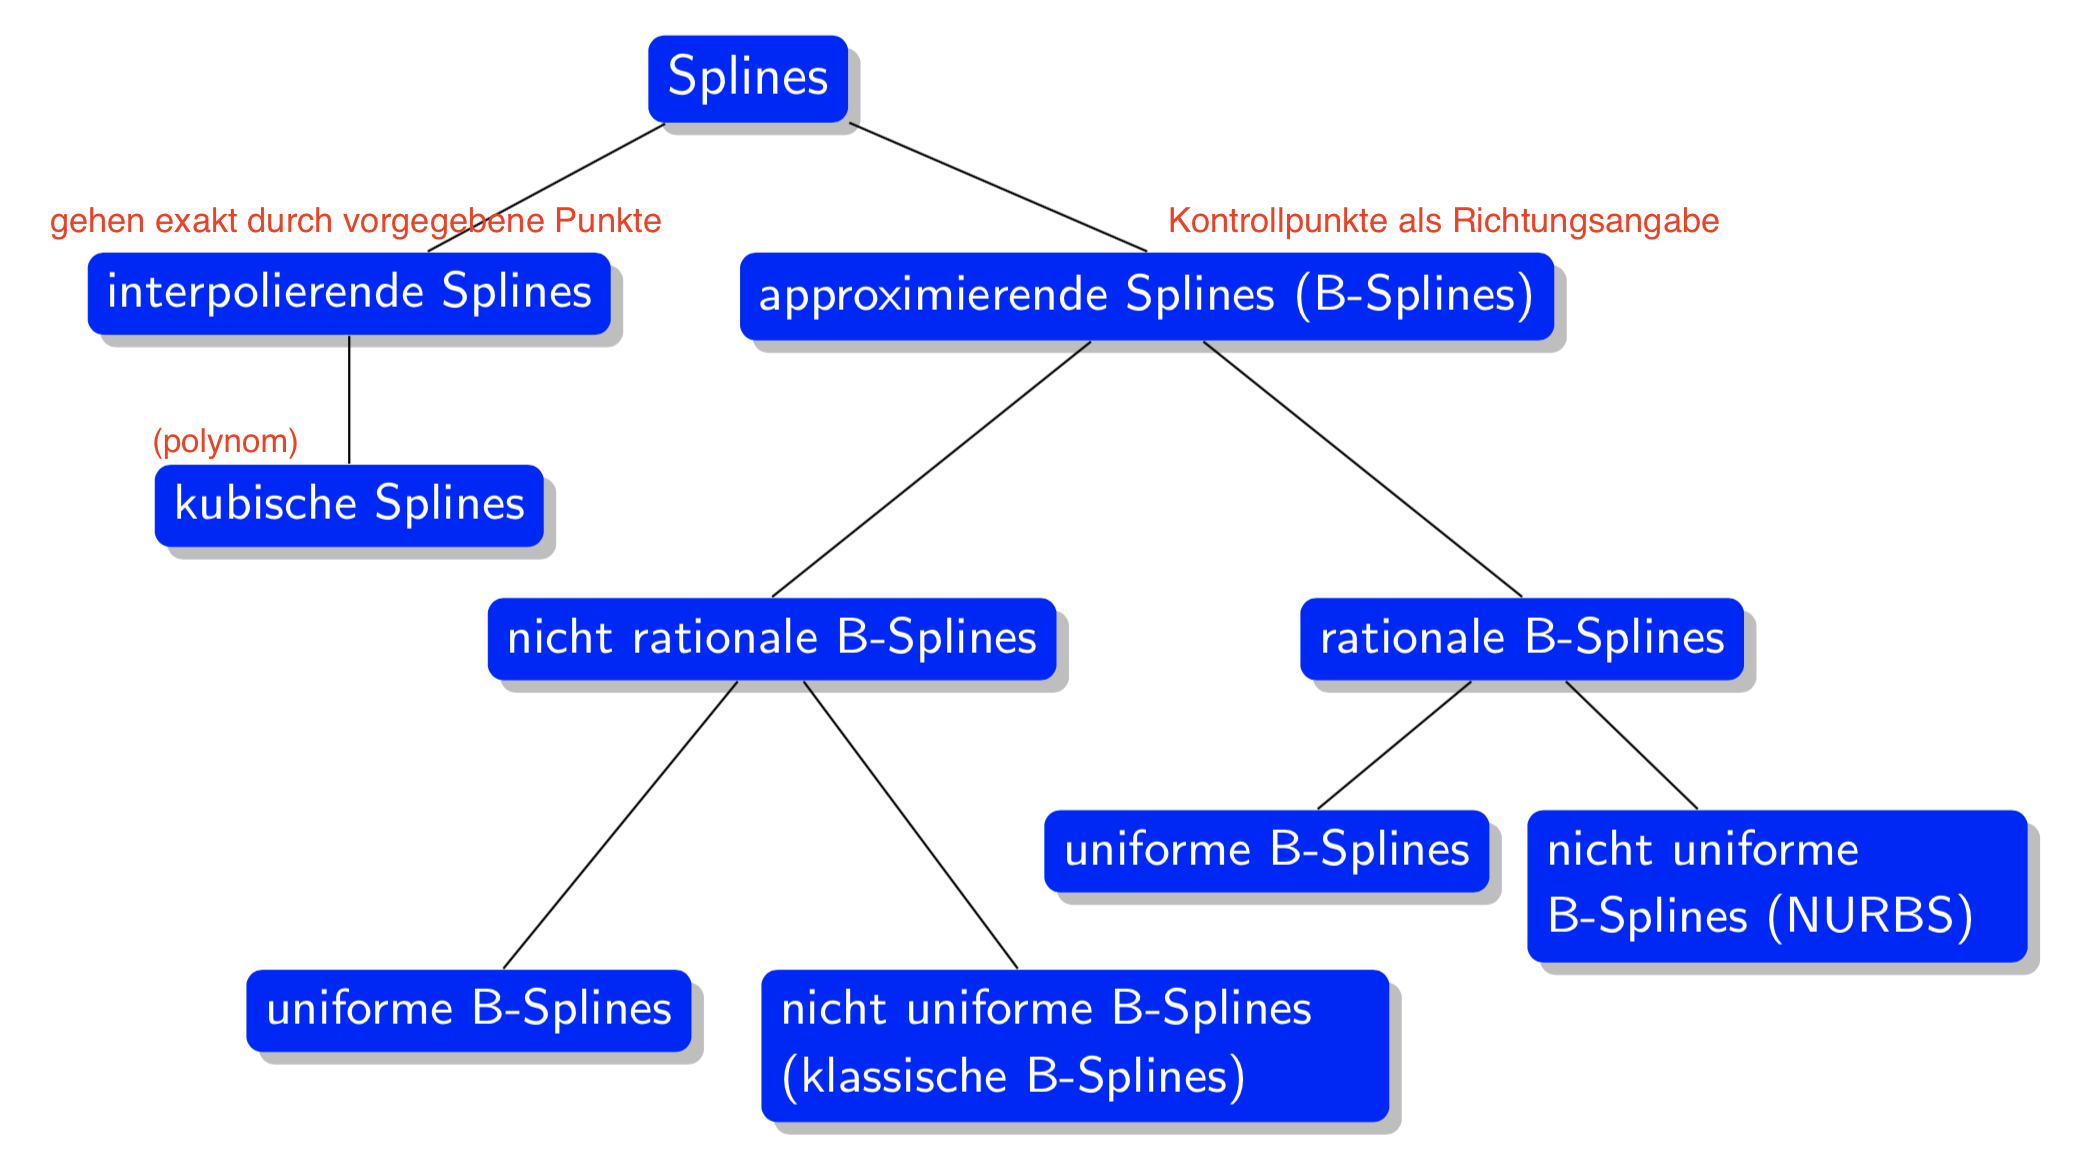
\includegraphics[width=0.5\textwidth]{assets/InterpolationVSApproximation.png}


\subsection{Methode unbestimmte Koeffizienten (Interpolation)}
TODO Beschreibung
$P_3(x) = c_0 + c_1x^2 + c_2x^2 + c_3x^3$ \\
\\
$\begin{bmatrix}
    1 & x_0 & x_0^2 & x_0^3 \\
    1 & x_1 & x_1^2 & x_1^3 \\
    1 & x_2 & x_2^2 & x_2^3 \\
    1 & x_3 & x_3^2 & x_3^3 \\
\end{bmatrix} 
\begin{bmatrix}
    c_0 \\
    c_1 \\
    c_2 \\
    c_3
\end{bmatrix} = 
\begin{bmatrix}
    y_0 \\
    y_1 \\
    y_2 \\
    y_3
\end{bmatrix}$ \\
\\
\textit{$c_0 = c_1 = c_2 = c_3 = 1$}

\subsection{Lagrange Methode (Interpolation)}

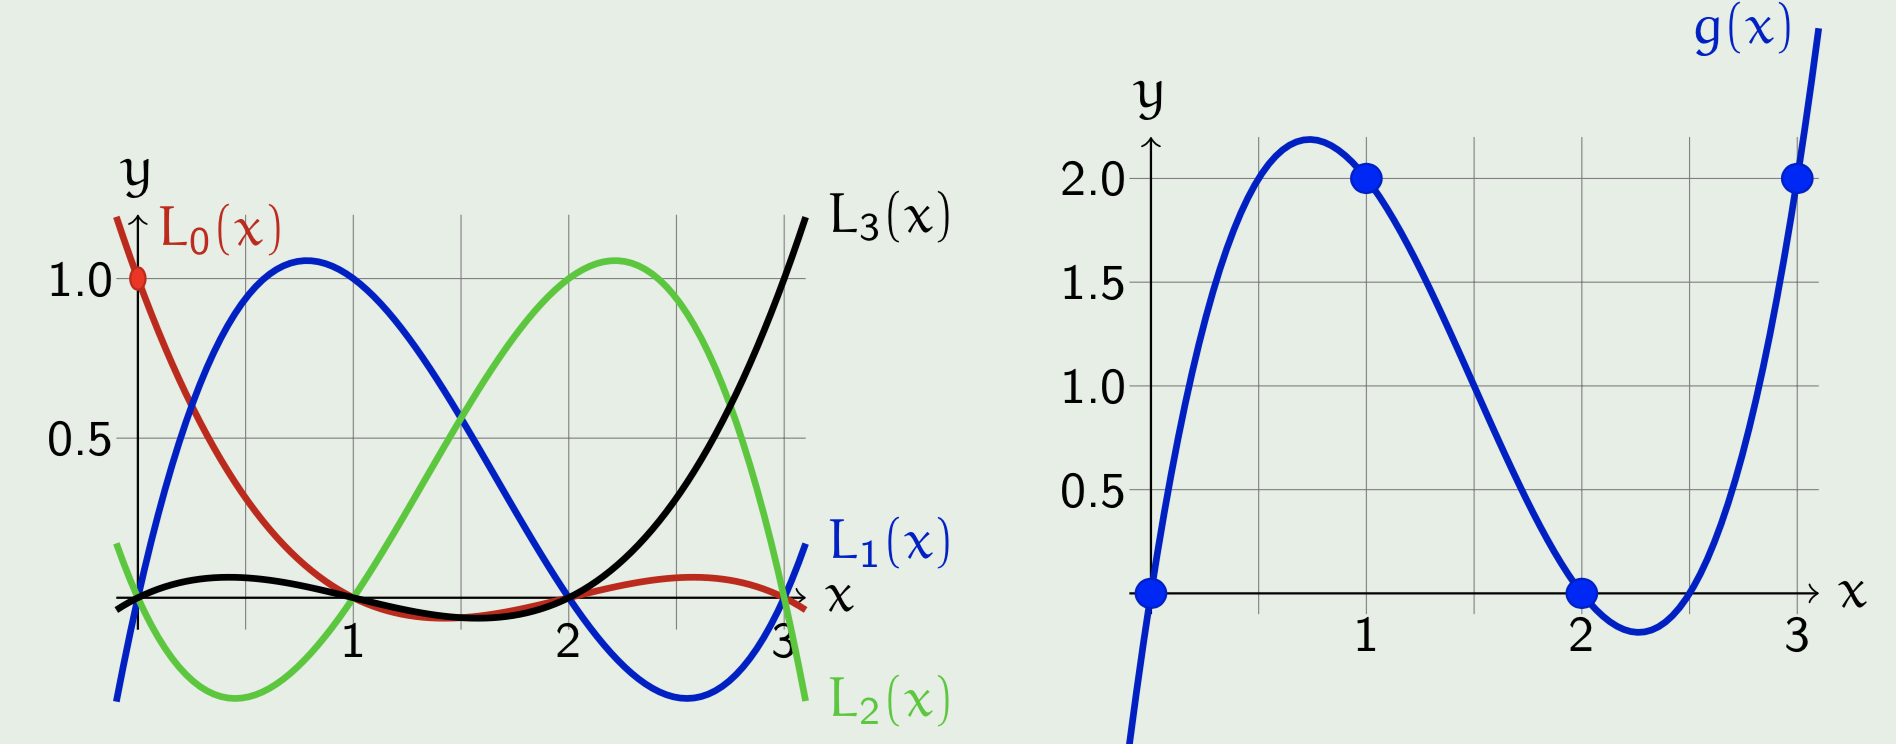
\includegraphics[width=0.5\textwidth]{assets/Lagrange1.png}
Polynome 3. Grades, welche an allen Stützstellen Null sind ausser an einer, wo der Wert Eins (1) sein soll:
$L_0(x) = \frac{(x-x_1)(x-x_2)(x-x_3)}{(x_0-x_1)(x_0-x_2)(x_0-x_3)}$ \\
$L_1(x) = \frac{(x-x_0)(x-x_2)(x-x_3)}{(x_1-x_0)(x_1-x_2)(x_1-x_3)}$ \\
$L_2(x) = \frac{(x-x_0)(x-x_1)(x-x_3)}{(x_2-x_0)(x_2-x_1)(x_2-x_3)}$ \\
$L_3(x) = \frac{(x-x_0)(x-x_1)(x-x_2)}{(x_3-x_0)(x_3-x_1)(x_3-x_2)}$ \\
\\
$g(x) = 0 \cdot L_0(x) + 2 \cdot L_1(x) + 0 \cdot L_2(x) + 2 \cdot L_3(x)$
\textit{Addition der einzelnen Polynome ergibt die gesuchte Kurve durch die vorgegebenen Punkte}\\
\\

TODO aufräumen:
$l_0(x) = (x-x_1)(x-x_2)\dots$ \\
$L_0(x) = \frac{l_0(x)}{l_0(x_0)} = \frac{(x-x_1)(x-x_2)\dots}{(x_0-x_1)(x_0-x_2)\dots}$ \\
$P_n(x) = y_0L_0(x)+y_1L_1(x)+ \dots + y_nL_n()$ \\
\\
\textit{Funktionen an den Stützstellen entweder Null oder Eins}
$l_k(x) = \prod^{n}_{i=0 \\ i \neq k}(x-x_i)$ \\
$L_k(x) = \frac{l_k(x)}{l_k(x_k)}$

\subsection{Lineare Bézier spline (Approximation)}

$P(0)$ \textit{= Anfang}\\
$P(1)$ \textit{= Ende}\\
\\
$P(t) = (1 - t) P_0 + P_1 (0 \leq t \leq 1)$ \\
\textit{Gewichteter Durchschnitt der Kontrollpunkte} \\
\\
$P(t) = (P_1 - P_0) t + P_0$ \\
\textit{Polynom in $t$} \\
\\
$P(t) = [P_0, P_1] \begin{bmatrix}
    -1 & 1 \\ 1 & 0
\end{bmatrix}
\begin{bmatrix}
    t \\ 1
\end{bmatrix} (0 \leq t \leq 1)$ \\
\textit{Matrizform}

\subsection{Quadric Bézier spline (Approximation)}
\textit{Verhältniss der Linien ist immer gleich}\\
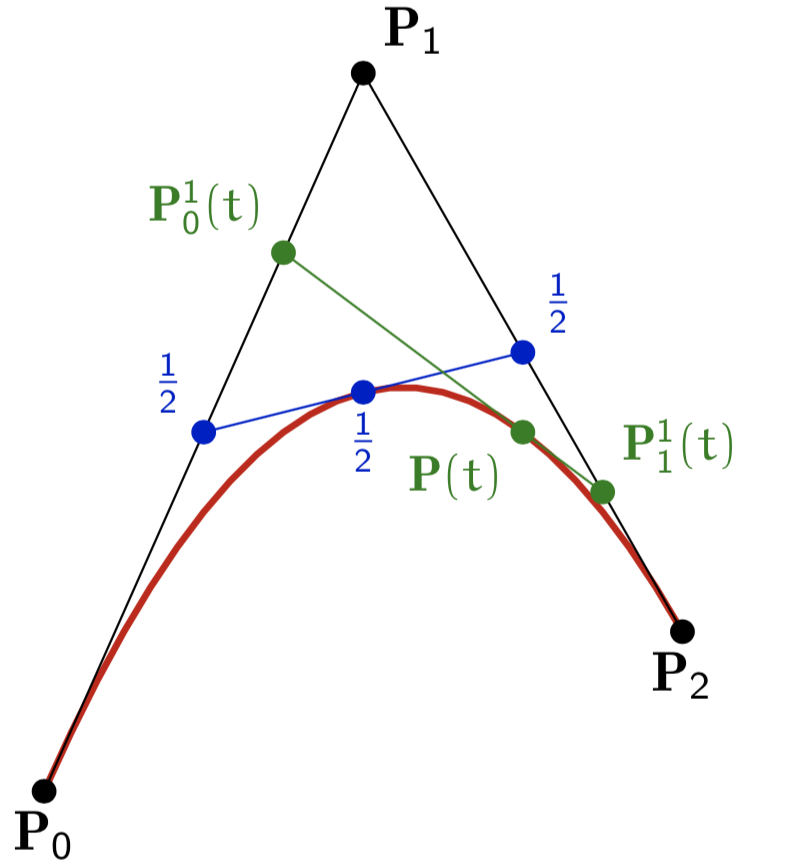
\includegraphics[width=0.3\textwidth]{assets/quadratischeBesierSpline.png}

\textit{drei Kontrollpunkte $P_0, P_1, P_2$}\\

$P_0^1(t) = (1-t)P_0 + P_1$ \\
$P_1^1(t) = (1-t)P_0 + P_1$ \\

$P(t) = (1 - t)^2P_0 + 2(1 - t)tP_1 + t^2 P_2$

\subsection{Qubic Bézier Spline (Approximation)}
\textit{Punkt = Punkt auf Linie zwischen zwei Hilfslinien}\\
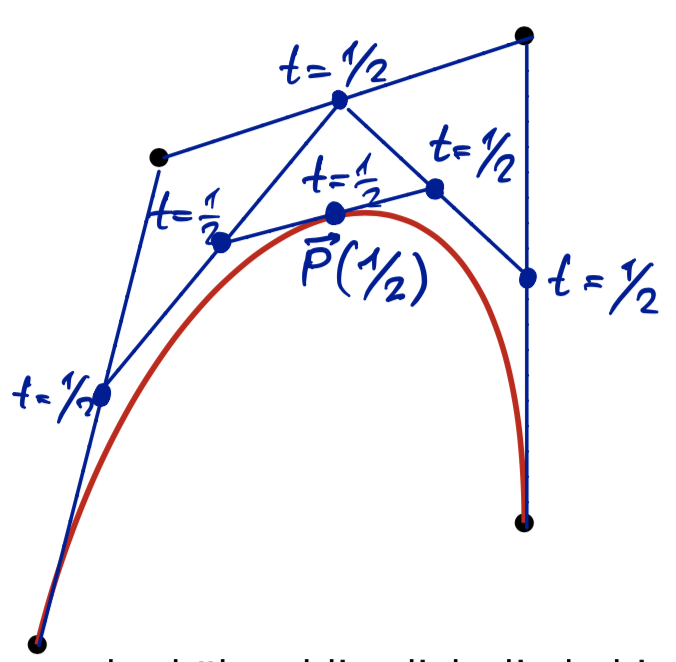
\includegraphics[width=0.3\textwidth]{assets/qubicBesierSpline.png}

\textit{vier Kontrollpunkte $P_0, P_1, P_2, P_3$}\\

\textit{Mit $P_0^1$, $P_1^1$ und} \\
$P_2^1(t) = (1-t)P_2 + tP_3$ \\

$P_1^2(t) = (1 - t) P_0^1(t) + tP_1^1(t)$ \\
$P_2^2(t) = (1 - t) P_1^1(t) + tP_2^1(t)$ \\

$P(t) = (1 - t)^3P_0 + 3(1 - t)^2tP_1 + 3(1 - t)t^2P_2 + t^3P_3$

\subsection{Bernsteinpolynome}
TODO

\subsection{Bézier-Kurven}
TODO
\textit{Kurve immer innerhalb der konvexen Hülle des Linienzuges der Kontrollpunkte}

\subsection{B-Spline-Kurven}
TODO
\begin{itemize}
	\item lokale Funktionen nur in der Nähe von Pj verschieden von 0 
	\item Einfluss vom Punkt auf die gesamte Kurve ist kleiner
\end{itemize}

\subsection{NURBS (Non Uniform Rational Basic Splines)}
TODO
\begin{itemize}
	\item homogenisiert
	\item rationale B-Spline-Kurve
	\item Punkte mit Gewichtung
	\item invariant bei den Transformationen
\end{itemize}